\documentclass{beamer}

% xcolor and define colors -------------------------
\usepackage{xcolor}

% https://www.viget.com/articles/color-contrast/
\definecolor{purple}{HTML}{5601A4}
\definecolor{navy}{HTML}{0D3D56}
\definecolor{ruby}{HTML}{9a2515}
\definecolor{alice}{HTML}{107895}
\definecolor{daisy}{HTML}{EBC944}
\definecolor{coral}{HTML}{F26D21}
\definecolor{kelly}{HTML}{829356}
\definecolor{cranberry}{HTML}{E64173}
\definecolor{jet}{HTML}{131516}
\definecolor{asher}{HTML}{555F61}
\definecolor{slate}{HTML}{314F4F}

% Mixtape Sessions
\definecolor{picton-blue}{HTML}{00b7ff}
\definecolor{violet-red}{HTML}{ff3881}
\definecolor{sun}{HTML}{ffaf18}
\definecolor{electric-violet}{HTML}{871EFF}

% Main theme colors
\definecolor{accent}{HTML}{00b7ff}
\definecolor{accent2}{HTML}{871EFF}
\definecolor{gray100}{HTML}{f3f4f6}
\definecolor{gray800}{HTML}{1F292D}


% Beamer Options -------------------------------------

% Background
\setbeamercolor{background canvas}{bg = white}

% Change text margins
\setbeamersize{text margin left = 15pt, text margin right = 15pt} 

% \alert
\setbeamercolor{alerted text}{fg = accent2}

% Frame title
\setbeamercolor{frametitle}{bg = white, fg = jet}
\setbeamercolor{framesubtitle}{bg = white, fg = accent}
\setbeamerfont{framesubtitle}{size = \small, shape = \itshape}

% Block
\setbeamercolor{block title}{fg = white, bg = accent2}
\setbeamercolor{block body}{fg = gray800, bg = gray100}

% Title page
\setbeamercolor{title}{fg = gray800}
\setbeamercolor{subtitle}{fg = accent}

%% Custom \maketitle and \titlepage
\setbeamertemplate{title page}
{
    %\begin{centering}
        \vspace{20mm}
        {\Large \usebeamerfont{title}\usebeamercolor[fg]{title}\inserttitle}\\
        {\large \itshape \usebeamerfont{subtitle}\usebeamercolor[fg]{subtitle}\insertsubtitle}\\ \vspace{10mm}
        {\insertauthor}\\
        {\color{asher}\small{\insertdate}}\\
    %\end{centering}
}

% Table of Contents
\setbeamercolor{section in toc}{fg = accent!70!jet}
\setbeamercolor{subsection in toc}{fg = jet}

% Button 
\setbeamercolor{button}{bg = accent}

% Remove navigation symbols
\setbeamertemplate{navigation symbols}{}

% Table and Figure captions
\setbeamercolor{caption}{fg=jet!70!white}
\setbeamercolor{caption name}{fg=jet}
\setbeamerfont{caption name}{shape = \itshape}

% Bullet points

%% Fix left-margins
\settowidth{\leftmargini}{\usebeamertemplate{itemize item}}
\addtolength{\leftmargini}{\labelsep}

%% enumerate item color
\setbeamercolor{enumerate item}{fg = accent}
\setbeamerfont{enumerate item}{size = \small}
\setbeamertemplate{enumerate item}{\insertenumlabel.}

%% itemize
\setbeamercolor{itemize item}{fg = accent!70!white}
\setbeamerfont{itemize item}{size = \small}
\setbeamertemplate{itemize item}[circle]

%% right arrow for subitems
\setbeamercolor{itemize subitem}{fg = accent!60!white}
\setbeamerfont{itemize subitem}{size = \small}
\setbeamertemplate{itemize subitem}{$\rightarrow$}

\setbeamertemplate{itemize subsubitem}[square]
\setbeamercolor{itemize subsubitem}{fg = jet}
\setbeamerfont{itemize subsubitem}{size = \small}







% Links ----------------------------------------------

\usepackage{hyperref}
\hypersetup{
  colorlinks = true,
  linkcolor = accent2,
  filecolor = accent2,
  urlcolor = accent2,
  citecolor = accent2,
}


% Line spacing --------------------------------------
\usepackage{setspace}
\setstretch{1.2}


% \begin{columns} -----------------------------------
\usepackage{multicol}


% Fonts ---------------------------------------------
% Beamer Option to use custom fonts
\usefonttheme{professionalfonts}

% \usepackage[utopia, smallerops, varg]{newtxmath}
% \usepackage{utopia}
\usepackage[sfdefault,light]{roboto}

% Small adjustments to text kerning
\usepackage{microtype}



% Remove annoying over-full box warnings -----------
\vfuzz2pt 
\hfuzz2pt


% Table of Contents with Sections
\setbeamerfont{myTOC}{series=\bfseries, size=\Large}
\AtBeginSection[]{
        \frame{
            \frametitle{Roadmap}
            \tableofcontents[current]   
        }
    }


% Tables -------------------------------------------
% Tables too big
% \begin{adjustbox}{width = 1.2\textwidth, center}
\usepackage{adjustbox}
\usepackage{array}
\usepackage{threeparttable, booktabs, adjustbox}
    
% Fix \input with tables
% \input fails when \\ is at end of external .tex file
\makeatletter
\let\input\@@input
\makeatother

% Tables too narrow
% \begin{tabularx}{\linewidth}{cols}
% col-types: X - center, L - left, R -right
% Relative scale: >{\hsize=.8\hsize}X/L/R
\usepackage{tabularx}
\newcolumntype{L}{>{\raggedright\arraybackslash}X}
\newcolumntype{R}{>{\raggedleft\arraybackslash}X}
\newcolumntype{C}{>{\centering\arraybackslash}X}

% Figures

% \imageframe{img_name} -----------------------------
% from https://github.com/mattjetwell/cousteau
\newcommand{\imageframe}[1]{%
    \begin{frame}[plain]
        \begin{tikzpicture}[remember picture, overlay]
            \node[at = (current page.center), xshift = 0cm] (cover) {%
                \includegraphics[keepaspectratio, width=\paperwidth, height=\paperheight]{#1}
            };
        \end{tikzpicture}
    \end{frame}%
}

% subfigures
\usepackage{subfigure}


% Highlight slide -----------------------------------
% \begin{transitionframe} Text \end{transitionframe}
% from paulgp's beamer tips
\newenvironment{transitionframe}{
    \setbeamercolor{background canvas}{bg=accent!40!black}
    \begin{frame}\color{accent!10!white}\LARGE\centering
}{
    \end{frame}
}


% Table Highlighting --------------------------------
% Create top-left and bottom-right markets in tabular cells with a unique matching id and these commands will outline those cells
\usepackage[beamer,customcolors]{hf-tikz}
\usetikzlibrary{calc}
\usetikzlibrary{fit,shapes.misc}

% To set the hypothesis highlighting boxes red.
\newcommand\marktopleft[1]{%
    \tikz[overlay,remember picture] 
        \node (marker-#1-a) at (0,1.5ex) {};%
}
\newcommand\markbottomright[1]{%
    \tikz[overlay,remember picture] 
        \node (marker-#1-b) at (0,0) {};%
    \tikz[accent!80!jet, ultra thick, overlay, remember picture, inner sep=4pt]
        \node[draw, rectangle, fit=(marker-#1-a.center) (marker-#1-b.center)] {};%
}

\usepackage{breqn} % Breaks lines

\usepackage{amsmath}
\usepackage{mathtools}

\usepackage{pdfpages} % \includepdf

\usepackage{listings} % R code
\usepackage{verbatim} % verbatim

% Video stuff
\usepackage{media9}

% packages for bibs and cites
\usepackage{natbib}
\usepackage{har2nat}
\newcommand{\possessivecite}[1]{\citeauthor{#1}'s \citeyearpar{#1}}
\usepackage{breakcites}
\usepackage{alltt}

% tikz
\usepackage{tikz}
\usepackage{pgfplots}
\usetikzlibrary{calc, positioning, decorations.pathreplacing, arrows.meta, intersections}
\pgfdeclarelayer{bg}
\pgfdeclarelayer{back}
\pgfdeclarelayer{fg}
\pgfsetlayers{bg,main,fg,back}
\usetikzlibrary{shapes,arrows}

% Setup math operators
\DeclareMathOperator{\E}{E} \DeclareMathOperator{\tr}{tr} \DeclareMathOperator{\se}{se} \DeclareMathOperator{\I}{I} \DeclareMathOperator{\sign}{sign} \DeclareMathOperator{\supp}{supp} \DeclareMathOperator{\plim}{plim}
\DeclareMathOperator*{\dlim}{\mathnormal{d}\mkern2mu-lim}
\newcommand\independent{\protect\mathpalette{\protect\independenT}{\perp}}
   \def\independenT#1#2{\mathrel{\rlap{$#1#2$}\mkern2mu{#1#2}}}
\newcommand*\colvec[1]{\begin{pmatrix}#1\end{pmatrix}}

\newcommand{\myurlshort}[2]{\href{#1}{\textcolor{gray}{\textsf{#2}}}}


\begin{document}

\imageframe{./lecture_includes/mixtape_ci_cover.png}


% ---- Content ----


\section{Introduction to course}

\subsection{What is Mixtape Sessions?}


\begin{frame}{Welcome!}

  \begin{itemize}
	\item Scott Cunningham, professor of economics at Baylor University, author of \underline{Causal Inference: the Mixtape}
	\item I run workshops on causal inference all over the world, but I am not an econometrician -- I'm a run of the mill applied microeconomist who studies severe mental illness who just happens to love learning and teaching
	\item Workshops can be helpful ways to plug into one's methodological training, and online workshops are very helpful because of the recordings, the coding together, and bunch of bells and whistles (e.g., github repositories)
	\item Causal inference is an old field but which has increasingly drawn people to it (Nobel Prize two years ago maybe helped) 
  \end{itemize}

\end{frame}



\begin{frame}{What is Mixtape Sessions?}

  \begin{itemize}
    \item Mixtape Sessions is my online platform started in November 2022 to ``democratize causal inference'' by helping connect people, from beginner to advanced, with material and teachers that for various reasons may not be accessible otherwise
    \item I became obsessed with teaching and writing about causal inference because of a strong conviction that (a) it is important and (b) not everyone had the same chances to learn it
    \item I wrote a 3-part sociological history of it on my substack that I encourage you to read so you can better understand the context for why I say that
    \item I tend to emphasize intuition, mechanics, narrow calculations, meaning, assumptions, code including actually taking time to code, advocate for data visualization -- in other words the art and the science
  \end{itemize}

\end{frame}

\begin{frame}{4-day Causal Inference Workshop}

  \begin{itemize}
    \item We workshop together for 4-days, 8am to 5pm CST, with 15 min breaks on the hour and a 1-hour lunch break at 12:00PM CST
    \item I mix exposition, discussion of papers, coding exercises and discussion as best as I can
    \item I'm me, and I teach how I teach, with passion, enthusiasm, deep joy, but I'm not an econometrician so sometimes I take the long way to get there when an econometrician would do it much faster
  \end{itemize}

\end{frame}

\subsection{Managing your expectations}

\begin{frame}{Class goals}

  \begin{enumerate}
    \item \textbf{Confidence}: You will feel like you have a good understanding of causal inference so that by the end it doesn't feel all that mysterious or intimidating
    \item \textbf{Comprehension}: You will have learned a lot both conceptually and in the specifics, particularly with regards to issues around identification and estimation
    \item \textbf{Competency}: You will have more knowledge of programming syntax in Stata and R (and python!) so that later you can apply this in your own work
  \end{enumerate}

\end{frame}


%\begin{frame}{Causal Inference table of contents}
%  \centering
%  \includegraphics[scale=0.5,height=6.5cm, width=10cm]{./lecture_includes/part1}
%\end{frame}

%\begin{frame}{Causal Inference Part 2}
%  \centering
%  \includegraphics[scale=0.5,height=6.5cm, width=10cm]{./lecture_includes/part2}
%  \url{https://www.mixtapesessions.io/session/ci_II_aug20}
%\end{frame}




\begin{frame}{Github repo}

  \begin{itemize}
    \item We will communicate with one another regularly in the Discord channel and I will always be monitoring it
    \item Encourage you to talk to each other there, help one another, network with one another, coauthor with one another!
    \item I will be distributing things to you, like code and slides, via the github repo: \url{github.com/Mixtape-Sessions/Causal-Inference-1}
    \item Each lecture will be recorded and then uploaded to Vimeo as a password protected file that you'll have access to into perpetuity
    \item Kyle Butts and I are committed to over time making the Github Repository like an open public library where the only club goods are (a) recordings, (b) Discord and (c) live lectures
  \end{itemize}

\end{frame}

\begin{frame}{Workshop (Part 1) Topics}

  \begin{enumerate}
    \item Foundations: Day 1
    \item Graphs and Selection on Observables: Day 2
    \item Instrumental Variables: Day 3
    \item Regression Discontinuity Design: Day 4
  \end{enumerate}

\end{frame}

\begin{frame}{Today: Day 1}

\begin{enumerate}
\item Potential outcomes
\item Randomization inference
\item Directed acyclic graphs
\end{enumerate}

\end{frame}

\subsection{Future Tracks}

\begin{frame}{Causal Inference Part 2}
  \centering
  \includegraphics[scale=0.5,height=6.5cm, width=10cm]{./lecture_includes/causal_part2a}
\end{frame}

\begin{frame}{Causal Inference Part 2}
  \centering
  \includegraphics[scale=0.5,height=6.5cm, width=10cm]{./lecture_includes/causal_part2b}
\end{frame}

\begin{frame}{Machine Learnings and Causal Inference}
  \centering
  \includegraphics[scale=0.5,height=6.5cm, width=10cm]{./lecture_includes/brigham_part1a}
\end{frame}

\begin{frame}{Machine Learnings and Causal Inference}
  \centering
  \includegraphics[scale=0.5,height=6.5cm, width=10cm]{./lecture_includes/brigham_part1b}
\end{frame}

\begin{frame}{Advanced DID}
  \centering
  \includegraphics[scale=0.5,height=6.5cm, width=10cm]{./lecture_includes/roth_part1a}
\end{frame}

\begin{frame}{Advanced DID}
  \centering
  \includegraphics[scale=0.5,height=6.5cm, width=10cm]{./lecture_includes/roth_part1b}
\end{frame}

\begin{frame}{Doing Applied Research}
  \centering
  \includegraphics[scale=0.5,height=6.5cm, width=10cm]{./lecture_includes/doing_part1a}
\end{frame}

\begin{frame}{Doing Applied Research}
  \centering
  \includegraphics[scale=0.5,height=6.5cm, width=10cm]{./lecture_includes/doing_part1b}
\end{frame}


\begin{frame}{Synthetic control and Clustering}
  \centering
  \includegraphics[scale=0.5,height=6.5cm, width=10cm]{./lecture_includes/abadie_part1a}
\end{frame}

\begin{frame}{Synthetic control and Clustering}
  \centering
  \includegraphics[scale=0.5,height=6.5cm, width=10cm]{./lecture_includes/abadie_part1b}
\end{frame}

\begin{frame}{Heterogenous treatment effects and machine learning}
  \centering
  \includegraphics[scale=0.5,height=6.5cm, width=10cm]{./lecture_includes/brigham_part2a}
\end{frame}

\begin{frame}{Heterogenous treatment effects and machine learning}
  \centering
  \includegraphics[scale=0.5,height=6.5cm, width=10cm]{./lecture_includes/brigham_part2b}
\end{frame}
















\section{Potential outcomes}



\subsection{Naive causal inference}


\begin{frame}{Coming to causal inference}

\begin{itemize}
\item Many roads lead to this material -- from computer science, to statistics, to economics, to philosophy, to epidemiology and so on and so forth
\item Therefore any effort to teach it will always have a degree of subjectivity reflecting the presenter
\item But even on something as narrow as what I'm going to discuss, there are even subtleties I want to take note of, and this reflects my own subjectivity

\end{itemize}

\end{frame}


\begin{frame}{Sociological history of causal inference}

\begin{itemize}

\item You can get a sense of my own perspective in my 3-part substack series on the sociological history of late 20th century quantitative causal inference (\url{https://causalinf.substack.com/p/a-selected-history-of-quantitative})
\item I'm not going to review it here, as it takes a long time, but I encourage you to read it as it can help you understand where this came from and why it looks the way it does, but also my own beliefs
\item All I will say is in my opinion, causal inference in the applied social sciences has two parents -- the statistician/econometricians and the ``ordinary data workers'' -- and that gives it the shape it has taken on
\end{itemize}

\end{frame}


\begin{frame}{Spurious correlations}
  \centering
  \includegraphics[scale=0.5,height=6.5cm, width=10cm]{./lecture_includes/spurious_correlation}
\end{frame}

\begin{frame}{Spurious correlations}

\begin{itemize}

\item What is causality?  \textbf{We need a definition}.
\item Philosophers created a definition, but statisticians found a trick to make it tractable
\item That trick combined notation (a definition) and a mechanism (treatment assignment) into ``acceptable solutions''
\item Let's now dig into the issues around definitions and then the first major breakthrough -- randomization

\end{itemize}

\end{frame}

\begin{frame}{Causality, causal inference}

\begin{itemize}

\item Philosophers have been interrogating what causality is going back to antiquity
\item It is one of the most important topics in both the fields of epistemology (how do I know if something causes something else?) and metaphysics (we will see why it involved metaphysics)
\item But I want you to distinguish for this workshop between the topic of ``causality'' and the topic of ``causal inference'', because the former is a much broader topic that includes many differing views
\item The latter is really a description of contemporary scientific methods bridging many sciences, including medicine, computer science, and much of the social sciences

\end{itemize}

\end{frame}

\begin{frame}{Philosophical origins of causal inference concepts}

  \begin{quote}
    ``If a person eats of a particular dish, and dies in consequence, that is, would not have died if he had not eaten it, people would be apt to say that eating of that dish was the source of his death.'' -- John Stuart Mill (19th century moral philosopher and economist)
  \end{quote}

  \bigskip
  
    \begin{quote}
    ``Causation is something that makes a difference, and the difference it makes must be a difference from what would have happened without it.'' -- David Lewis (20th century metaphysical philosopher)
  \end{quote}

\end{frame}



\begin{frame}{Ancient One explains it}

  Both people pinned the idea of causality in \emph{comparisons} between (1) different actions taken and (2) different timelines
  
  \bigskip
  
  Let's start off and listen to the Ancient One explain to Bruce Banner (aka the Incredible Hulk) from \underline{Avengers: Endgame}
  
  \bigskip
  
  \url{https://youtu.be/1S3I0PqkooA?t=50}
  
  \end{frame}
  
  \begin{frame}{Counterfactuals}
  
  Philosophers and stories alike eventually settled on the idea that causality was rooted in a particular kind of comparison, like ``treatment'' versus ``control'' groups
  
  \bigskip
  
  But the comparison as you heard the Ancient One say was much weirder than comparing two groups -- it was comparing two possible events (choices) across two possible timelines that may (or may not) trigger two different outcomes
  
  \bigskip
  
  The key idea in contemporary causal inference is the idea of the counterfactual. Counterfactuals are neither past nor future.  They are alternative histories created by thought experiments but we use them as framing devices to decipher causality in our timeline

\end{frame}

\begin{frame}{Statistical origins}

\begin{quote}
``Yet, although the seeds of the idea that [causal effects are comparisons of potential outcomes] can be traced back at least to the 18th century [most likely he means David Hume], the formal notation for potential outcomes was not introduced until 1923 by Neyman.'' -- Don Rubin (1990)
\end{quote}

\end{frame}


\begin{frame}{Jerzy Neyman introduces his definition}

\begin{itemize}
\item Early 20th century statistician, one of the ``fathers'' of modern statistics
\item 1923 article describes a field experiment with differing plots of land (imagine hundreds of square gardens) and many different ``varieties'' of fertilizer that farmers could apply to the land
\item ``$U_{ik}$ is the yield of the $i$th variety on the $k$th plot...'' (Neyman 1923)
\item He calls $U_{ik}$ ``potential yield'', as opposed to the realized yield because $i$ (the fertilizer type) described all possible fertilizers that could be assigned to each $k$ square garden
\item Though only one fertilizer will be assigned to the land, many possibilities exist in other words
\end{itemize}

\end{frame}

\begin{frame}{Urn model}

\begin{itemize}

\item For each fertilizer there is an associated ``potential yield'' that he collapses into $U$ and each of them he considers to be ``a priori fixed but unknown'' (Rubin 1990)
\item Farmers draw fertilizer from an urn, like a bingo ball from a bingo ball machine, and apply it to each square garden
\item Once the fertilizer is assigned, we go from ``all possible outcomes'' to ``realized outcome'' terminology
\item Interestingly -- the urn model was a thought experiment, but it was stochastically identical to the completely randomized experiment, and he doesn't notice it
\item His arch-rival, Ronald Fisher, does notice it and publishes a book two years later recommending randomized experiments rooted in this paper
\end{itemize}

\end{frame}

\begin{frame}{Treatment assignment mechanism}

\begin{quote}

``Before the 20th century, there appears to have been only limited awareness of the concept of the assignment mechanism.  Although by the 1930s, randomized experiments were firmly established in some areas of scientific investigation, notably in agricultural experiments, there was no formal statement for a general assignment mechanism and, moreover, not even formal arguments in favor of randomization until Fisher (1925).'' (Imbens and Rubin 2015)

\end{quote}

\end{frame}

\begin{frame}{Progress is made and progress is not made}

\begin{itemize}

\item Whereas the RCT takes off in medicine and agriculture, it is not adopted as universally in social sciences, like economics
\item Economics ironically does have in its history early econometricians who thought about causality like Neyman and Fisher, but listen to Guido Imbens describe the transition towards modeling causality in terms of ``realized outcomes

\end{itemize}

\bigskip

\url{https://www.youtube.com/watch?v=drGkRy53bB4}

\end{frame}

\begin{frame}{Prediction vs causal inference}

\begin{itemize}

\item Statistics was not merely interested in causal inference
\item It was also interested in prediction, as are many of the social sciences
\item But causal inference appeared to progress from Neyman-Fisher until Rubin's 1970s work without explicit references to Neyman's original ideas
\item I think sometimes therefore the ``clarity'' as Imbens said was lost and as such, prediction and causal inference did not have sharp lines separating them

\end{itemize}

\end{frame}

\begin{frame}{Different types of prediction}

  \begin{columns}
    \column{0.48\linewidth}
    \centering
    \textbf{Traditional prediction}
    \begin{itemize}
      \item Traditional prediction seeks to detect patterns in data and fit functional relationships between variables with a high degree of accuracy
      \item ``Does this person have heart disease?'', ``How many books will I sell?''
      \item It is not predictions of what effect a choice will have, though
    \end{itemize}
    \column{0.48\linewidth}
    \centering
    \textbf{Causal inference}
    \begin{itemize}
      \item Causal inference is also a type of prediction, but it's a prediction of a \emph{counterfactual} associated with a particular \emph{choice taken}
      \item Causal inference takes that predicted (or imputed) counterfactual and constructs a causal effect that we hope tells us about a future in the event of a similar choice taken
    \end{itemize}
  \end{columns}
\end{frame}


\begin{frame}{Identification problem}
  \centering
  \includegraphics[scale=0.5,height=6.5cm, width=10cm]{./lecture_includes/prediction_causality.png}
\end{frame}




\begin{frame}{Naive causal inference}

  \begin{itemize}
    \item Aliens come and orbit earth, see people dying in hospitals and conclude ``doctors are hurting people''
    \item They kill the doctors, unplug patients from machines, throw open the doors -- many patients inexplicably die
    \item \emph{We are the aliens in our research}
  \end{itemize}

\end{frame}

\begin{frame}{\#1: Correlation and causality are different concepts}

  Causal is one unit, correlation is many units
  \begin{itemize}
    \item Causal question: ``If a doctor puts a patient on a ventilator (D), will her covid symptoms (Y) improve?''
    \item Correlation question:  $$\frac{Cov(D,Y)}{\sqrt{Var_D}\sqrt{{Var_Y}}}$$
  \end{itemize}

\end{frame}


\begin{frame}{\#2: Coming first may not mean causality!}

  \begin{itemize}
    \item Every morning the rooster crows and then the sun rises
    \item Did the rooster cause the sun to rise? Or did the sun cause the rooster to crow?
    \item What if cat killed the rooster?
    \item \emph{Post hoc ergo propter hoc}: ``after this, therefore, because of this''
  \end{itemize}

\end{frame}

\begin{frame}{\#3: Causality may mask correlations!}

  \begin{figure}
    \centering
    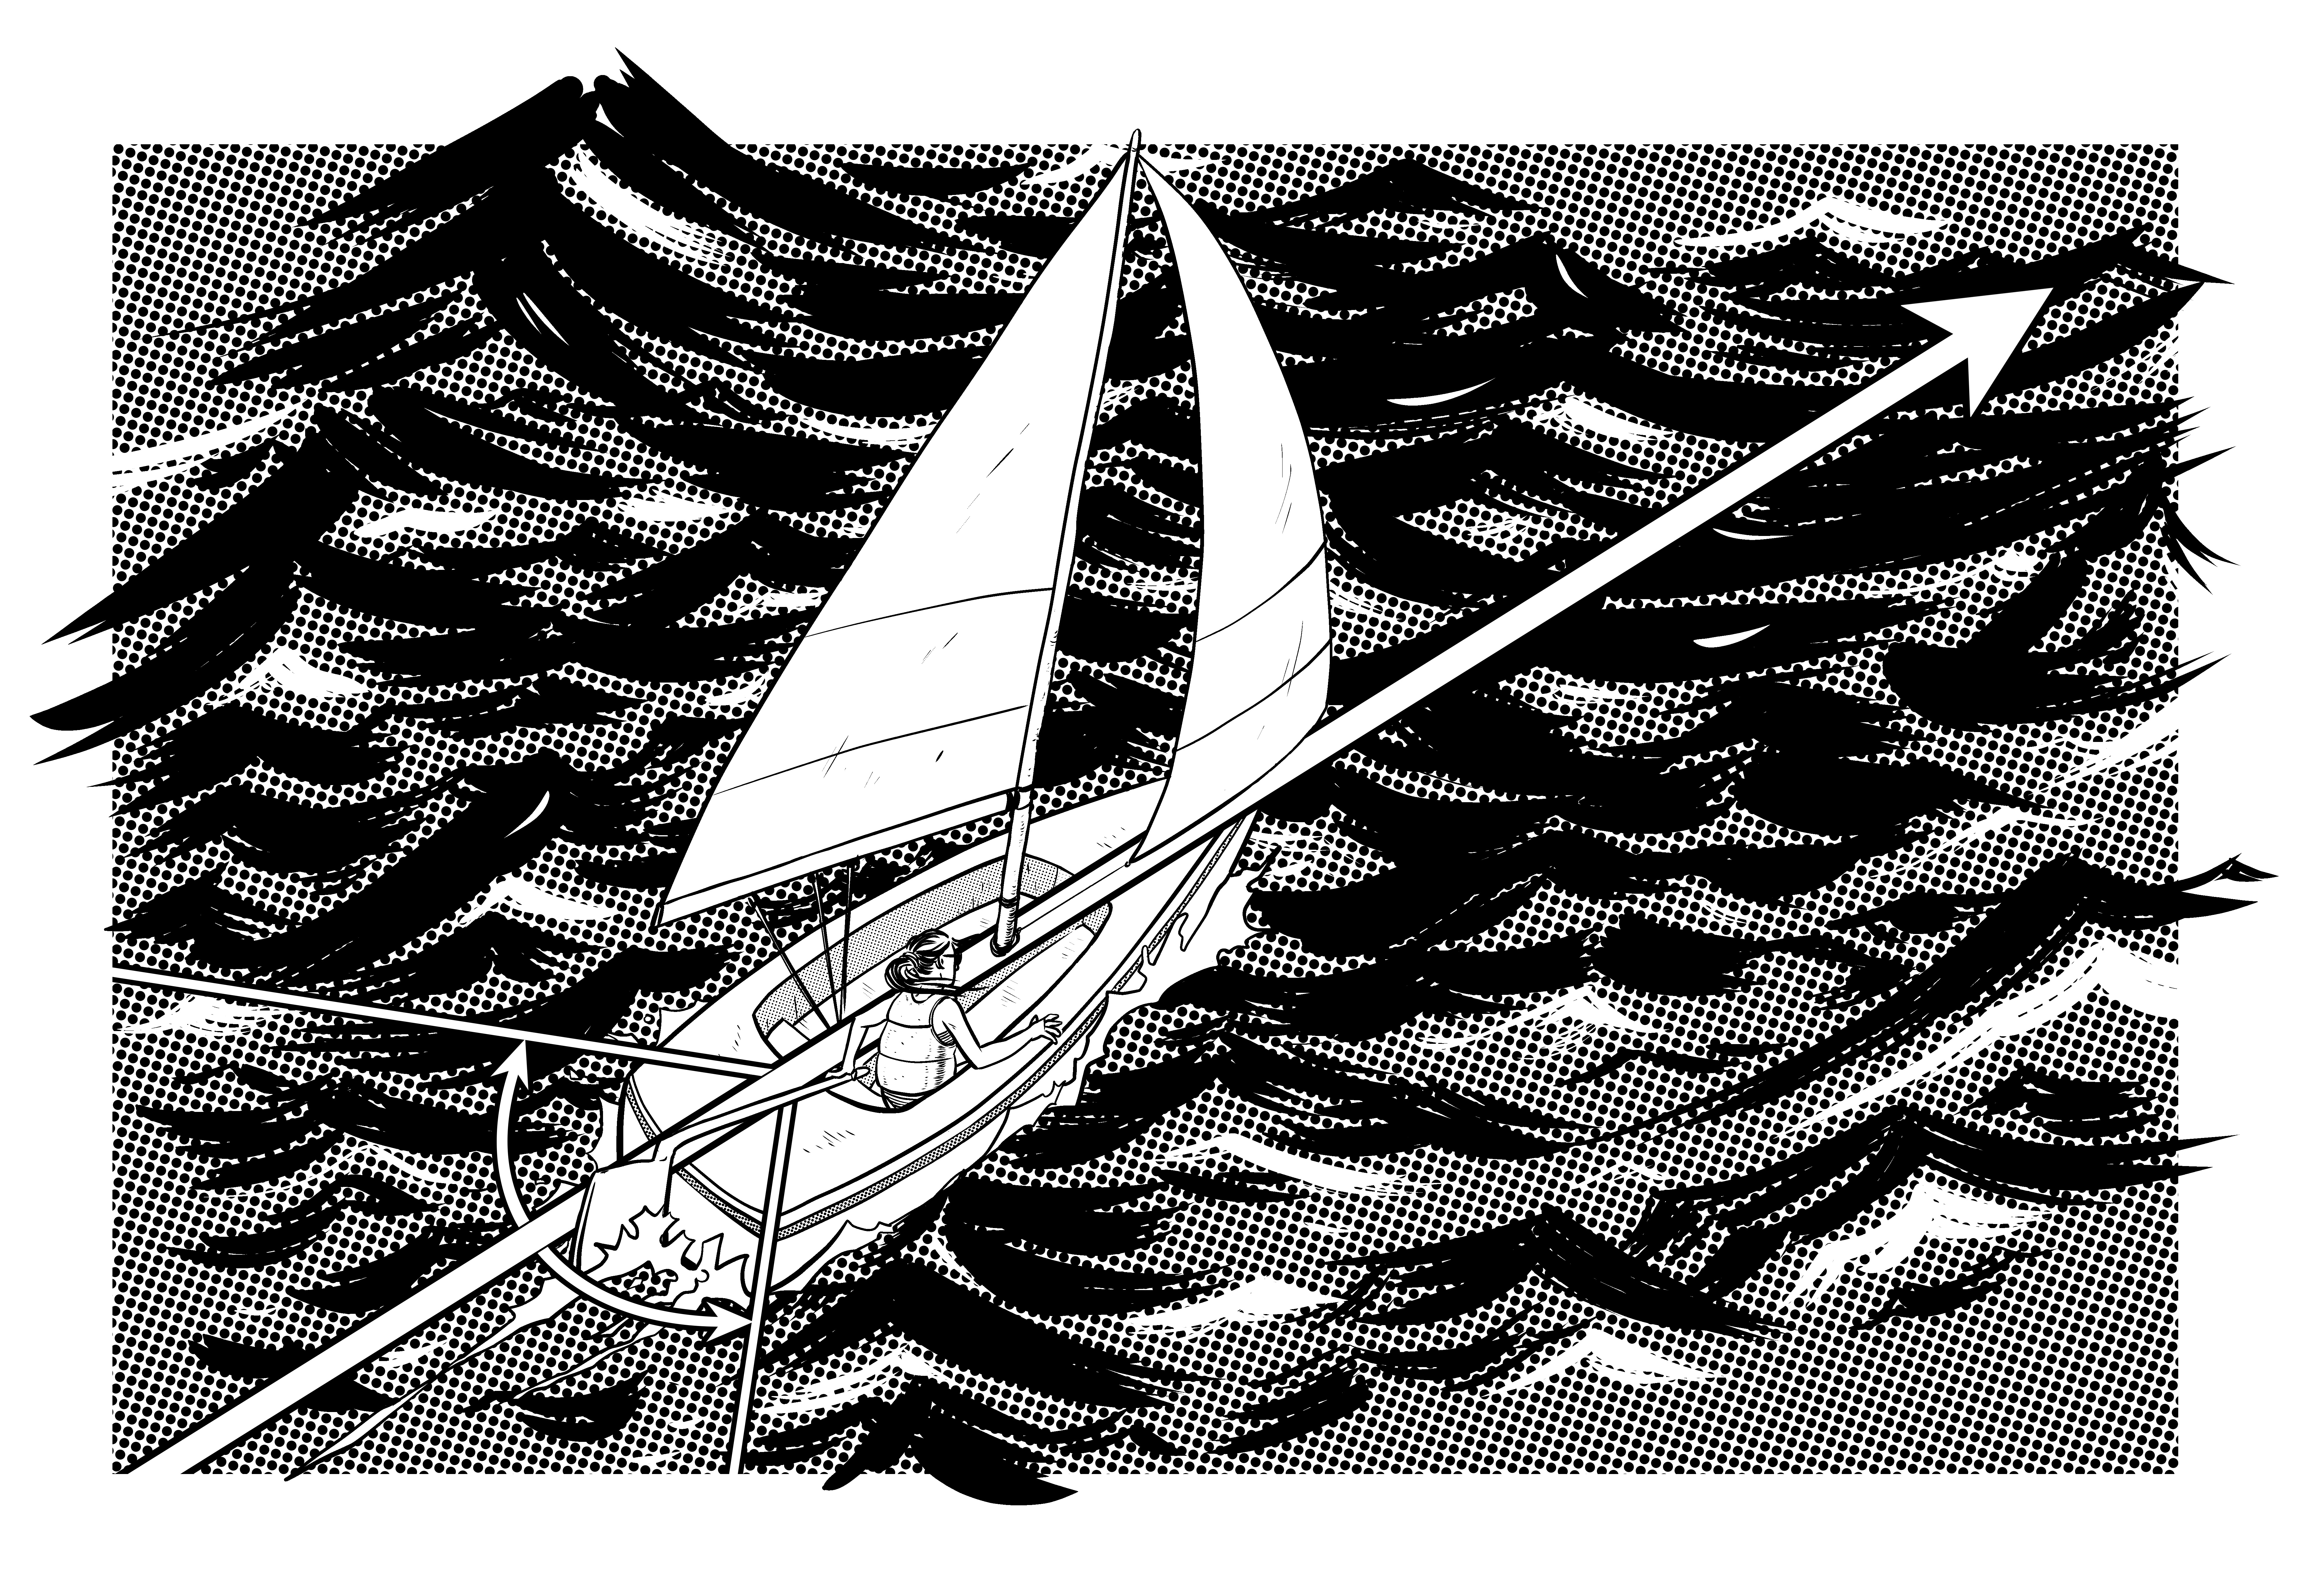
\includegraphics[scale=0.04]{./lecture_includes/scottboat.jpg}
  \end{figure}

\end{frame}


\subsection{Potential outcomes notation}





\begin{frame}{Potential outcomes notation}

  \begin{itemize}
    \item Let the treatment be a binary variable: $$D_{i,t} =\begin{cases} 1 \text{ if placed on ventilator at time $t$} \\ 0 \text{ if not placed on ventilator at time $t$} \end{cases}$$where $i$ indexes an individual observation, such as a person
  \end{itemize}
\end{frame}

\begin{frame}{Potential outcomes notation}

  \begin{itemize}
    \item Potential outcomes: $$Y_{i,t}^j =\begin{cases} 1 \text{ health if placed on ventilator at time $t$} \\ 0 \text{ health if not placed on ventilator at time $t$} \end{cases}$$where $j$ indexes a potential treatment status for the same $i$ person at the same $t$ point in time
  \end{itemize}
\end{frame}


\begin{frame}{Realized vs potential outcomes}

  \begin{itemize}
    \item Potential outcomes $Y^1$ and realized outcomes $Y$ are not the same ideas or notation
    \item Potential outcomes refer to the ``a priori fixed but unknown'' outcomes associated with different possible treatment assignments
    \item Realized outcomes refer to the ``posterior and known'' outcome associated with a specific treatment assignment
    \item This distinction is more subtle than I can emphasize, and so we have to spend time on the front end in spreadsheets and code
  \end{itemize}
\end{frame}

\begin{frame}{Important definitions}

    \begin{block}{Definition 1: Individual treatment effect}
      The individual treatment effect,  $\delta_i$, associated with a ventilator is equal to $Y_i^1-Y_i^0$.
    \end{block}
\end{frame}


\begin{frame}{Important definitions}


    \begin{block}{Definition 2: Switching equation}
      An individual's realized health outcome, $Y_i$, is determined by treatment assignment, $D_i$ which selects one of the potential outcomes:
      \begin{eqnarray*}
        Y_i& = D_iY^1_i+(1-D_i)Y^0_i& \\
        Y_i& = \begin{cases}
          Y^1_i\text{ if }D_i=1 \\
          Y^0_i\text{ if }D_i=0
        \end{cases}
      \end{eqnarray*}
    \end{block}

\end{frame}


\begin{frame}{Missing data problem}


    \begin{block}{Definition 3: Fundamental problem of causal inference}
      If you need both potential outcomes to know causality with certainty, then since it is impossible to observe both $Y_i^1$ and $Y_i^0$ for the same individual, $\delta_i$, is \emph{unknowable}.
    \end{block}
    
      \begin{itemize}
    \item Fundamental problem of causal inference is a consequence of what the switching equation does and cannot be fixed with more data -- always missing one of the potential outcomes
    \item Causal inference is a missing data problem requiring imputation of missing counterfactuals (sometimes explicitly such as with nearest neighbor or synthetic control, sometimes implicitly as with RDD)
  \end{itemize}

    
\end{frame}



\begin{frame}{Average Treatment Effects}

  \begin{block}{Definition 4: Average treatment effect (ATE)}
    The average treatment effect is the population average of all $i$ individual treatment effects
    \begin{eqnarray*}
      E[\delta_i]&=&E[Y_i^1-Y_i^0]\\
      &=&E[Y^1_i] - E[Y^0_i]
    \end{eqnarray*}
  \end{block}

  \bigskip

Aggregate parameters based on individual treatment effects are \emph{summaries} of individual treatment effects

\bigskip

  Cannot be calculated because $Y^1_i$ and $Y^0_i$ do not exist \emph{for the same unit i} due to switching equation

\end{frame}



\begin{frame}{Conditional Average Treatment Effects}


  \begin{block}{Definition 5: Average Treatment Effect on the Treated (ATT)}
    The average treatment effect on the treatment group is equal to the average treatment effect conditional on being a treatment group member:
    \begin{eqnarray*}
      E[\delta|D=1]&=&E[Y^1-Y^0|D=1] \nonumber \\
      &=&E[Y^1|D=1]-E[Y^0|D=1]
    \end{eqnarray*}
  \end{block}
  Cannot be calculated because $Y^1_i$ and $Y^0_i$ do not exist \emph{for the same unit i} due to switching equation. 


\end{frame}



\begin{frame}{Conditional Average Treatment Effects}

  \begin{block}{Definition 6: Average Treatment Effect on the Untreated (ATU)}
    The average treatment effect on the untreated group is equal to the average treatment effect conditional on being untreated:
    \begin{eqnarray*}
      E[\delta|D=0]&=&E[Y^1-Y^0|D=0] \nonumber \\
      &=&E[Y^1|D=0]-E[Y^0|D=0]
    \end{eqnarray*}
  \end{block}
  Cannot be calculated because $Y^1_i$ and $Y^0_i$ do not exist \emph{for the same unit i} due to switching equation

\end{frame}


\begin{frame}{Any collection of treatment effects}

  \begin{itemize}
	\item Notice how in all three of these, all we did was take the defined treatment effect at the individual and aggregate
	\item The aggregate causal parameters are \emph{definitions} of summaries but cannot be calculated directly bc of missing data problem
	\item But they can be estimated, which is probably a distinction in epistemology as it's knowledge but of a different type (``warranted belief'')
  \end{itemize}

\end{frame}

\subsection{Selection bias}

\begin{frame}{Naive causal inference and selection bias}

  \begin{itemize}
    \item Naive causal inference is often caused by confusing prediction or description with causal inference
    \item It is naive if it does not directly address, in a reasonable way, the problem of \emph{selection bias}
    \item This is better seen with a story and a decomposition
  \end{itemize}

\end{frame}






\begin{frame}[plain]


  \begin{block}{Definition 7: Simple difference in mean outcomes (SDO)}
    A simple difference in mean outcomes (SDO) can be approximated by the sample averages:\begin{eqnarray*}
      SDO &=& E[Y^1 | D=1] - E[Y^0 | D=0] \\
      &=& E[Y | D=1] - E[Y | D=0]
    \end{eqnarray*}
  \end{block}
  \bigskip

Notice how I moved between potential outcomes ($Y^1$) to realized outcomes ($Y$ for $D=1$) using the switching equation

\end{frame}

\begin{frame}{Simple difference in mean outcomes}

  \begin{itemize}
    \item Simple difference in mean outcomes may or may not be ``naive''
    \item It can be calculated manually by differencing averages, or with a regression $$Y_i = \alpha + \delta D_i + \varepsilon_{i}$$where $\widehat{\delta}$ is the SDO from the previous slide
    \item SDO creates a number (i.e., it's a calculation), but what does that number mean in terms of causality and bias?
  \end{itemize}

\end{frame}


\begin{frame}{Decomposition of the SDO}

  \begin{block}{Decomposition of the SDO}
    The SDO is made up of three things:
    \begin{eqnarray*}
      E[Y^1 | D=1] - E[Y^0 | D=0]&=& ATE\nonumber \\
      &&+ E[Y^0|D=1] - E[Y^0|D=0] \nonumber \\
      && + (1-\pi)(ATT - ATU)
    \end{eqnarray*}
  \end{block}

\bigskip

We need to see this as everything hinges on getting it
\end{frame}


\begin{frame}{Begin with ATE definition}

  \begin{block}{Law of iterated expectations}
    \begin{eqnarray*}
      \text{ATE}&=&E[Y^1]-E[Y^0]  \\
      &=& \{\pi E[Y^1 | D=1] + (1-\pi)E[Y^1 | D=0]\}  \\
      & & - \{\pi E[Y^0|D=1] + (1-\pi) E[Y^0 | D=0]\}
    \end{eqnarray*}
  \end{block}



\end{frame}

\begin{frame}{Change notation}



  \begin{block}{Substitute letters for expectations to go easy on the eyes}
    \begin{eqnarray*}
      E[Y^1|D=1] &=& a  \\
      E[Y^1|D=0] &=& b  \\
      E[Y^0|D=1] &=& c  \\
      E[Y^0|D=0] &=& d  \\
      \text{ATE} &=& e
    \end{eqnarray*}
  \end{block}


\end{frame}

\begin{frame}{Rewrite ATE definition}


  \begin{block}{Rewrite ATE}
    \begin{eqnarray*}
      e&=&\{\pi{a} + (1-\pi)b\} - \{\pi{c} + (1-\pi)d\}
    \end{eqnarray*}
  \end{block}

\end{frame}




\begin{frame}[plain]

  \begin{block}{Simple manipulation of ATE definition}
    \begin{eqnarray*}
      e&=&\{\pi{a} + (1-\pi)b\} - \{\pi{c} + (1-\pi)d\}  \\
      e&=&\pi{a} + b - \pi{b} - \pi{c} - d + \pi{d}  \\
      e&=&\pi{a} + b - \pi{b} - \pi{c} - d + \pi{d} + (\textbf{a} - \textbf{a}) + (\textbf{c} - \textbf{c}) + (\textbf{d} - \textbf{d})  \\
      0&=&e-\pi{a} - b + \pi{b} + \pi{c} + d - \pi{d} - \textbf{a} + \textbf{a} - \textbf{c} + \textbf{c} - \textbf{d} + \textbf{d}  \\
      \textbf{a}-\textbf{d}&=&e-\pi{a} - b + \pi{b} + \pi{c} + d - \pi{d}  + \textbf{a} - \textbf{c} + \textbf{c} - \textbf{d}  \\
      \textbf{a}-\textbf{d}&=&e  + (\textbf{c} - \textbf{d}) + \textbf{a}-\pi{a} - b + \pi{b} - \textbf{c} + \pi{c} + d - \pi{d} \\
      \textbf{a}-\textbf{d}&=&e  + (\textbf{c} - \textbf{d}) + (1-\pi)a -(1-\pi)b + (1-\pi)d - (1-\pi)c  \\
      \textbf{a}-\textbf{d}&=&e  + (\textbf{c} - \textbf{d}) + (1-\pi)(a-c) -(1-\pi)(b-d)
    \end{eqnarray*}
  \end{block}


\end{frame}

\begin{frame}[shrink=20,plain]
  \begin{block}{Carry forward from previous slide}
    \begin{eqnarray*}
      \textbf{a}-\textbf{d}&=&e  + (\textbf{c} - \textbf{d}) + (1-\pi)(a-c) -(1-\pi)(b-d)
    \end{eqnarray*}
  \end{block}

  \begin{block}{Replace letters with original terms }
    \begin{eqnarray*}
      E[Y^1|D=1] - E[Y^0|D=0] &=& \text{ATE}  \\
      &&+ (E[Y^0|D=1] - E[Y^0|D=0])  \\
      && + (1-\pi)( \underbrace{\{E[Y^1|D=1] - \alert{E[Y^0|D=1]}\}}_{ \mathclap{\text{ATT}}}  \\
      && - (1-\pi)( \underbrace{\{E[Y^1|D=0] - \alert{E[Y^0|D=0]}\}}_{ \mathclap{\text{ATU}}}  \\
    \end{eqnarray*}
  \end{block}
\end{frame}

\begin{frame}{Decomposition of the SDO}

  \begin{block}{Decomposition of the SDO}
    \begin{eqnarray*}
      E[Y^1 | D=1] - E[Y^0 | D=0]  &=& ATE \\
      &&+ (E[Y^0|D=1] - E[Y^0|D=0])  \\
      && + (1-\pi)(ATT - ATU)
    \end{eqnarray*}
  \end{block}
  
  \bigskip
  
  Note: this is a \emph{rewritten} formula for the definition of the ATE and so is \emph{always} true.  Also, notice that we started with $\pi$ but in the end we weight by $1-\pi$.
\end{frame}


\begin{frame}[plain]

  \begin{block}{Estimate SDO with sample averages}
    \begin{eqnarray*}
      \underbrace{E_N[Y_i | D_i=1] - E_N[Y_i | D_i=0]}_{ \mathclap{\text{Estimate of SDO}}}&=& \underbrace{E[Y^1] - E[Y^0]}_{ \mathclap{\text{Average Treatment Effect}}} \\
      &&+ \underbrace{E[Y^0|D=1] - E[Y^0 | D=0]}_{ \mathclap{\text{Selection bias}}}  \\
      && + \underbrace{(1-\pi)(ATT - ATU)}_{ \mathclap{\text{Heterogenous treatment effect bias}}}
    \end{eqnarray*}
  \end{block}

\bigskip

    Using the switching equation and sample averages, we can calculate $E_N[Y|D=1] \to E[Y^1 | D=1]$, $E_N[Y|D=0] \to E[Y^0|D=0]$ and $(1-\pi)$ is the share of the population in the control group.

\end{frame}


\begin{frame}{Selection bias}

\begin{itemize}
\item For many of us, we have heard the word ``selection bias'' before but it was with respect to ``non-random samples''
\item In causal inference, that isn't what we mean.  We mean mean potential outcomes differ for two groups.
\item We cannot observe this though because one of the comparisons is counterfactual and the other is realized
\end{itemize}

\end{frame}

\begin{frame}{Bias \#1: Selection bias}

  \begin{itemize}
    \item Look very closely at the selection bias terms on their left and right hand sides $$E[Y^0|D=1] \neq E[Y^0 |D=0]$$
    \item Ask yourself: do you think that the people placed on vents would've had the same mean health outcomes as the people not on vents had they not been on vents? Why do you think that?
      \end{itemize}

\end{frame}

\begin{frame}{Bias \#1: Selection bias}

Probably not. Had they not been on vents, many would've died.

\bigskip

  $$\underbrace{E[Y^0|D=1]}_{\mathclap{\text{Worse off vents}}} < \underbrace{E[Y^0|D=0]}_{\mathclap{\text{Better off vents}}}$$

\bigskip

Bias was caused by \emph{the doctors} being good at their jobs!  

\bigskip

Bias was caused by the \emph{treatment assignment mechanism}, and Imbens and Rubin said that was not really emphasized until Fisher (1925) 


\end{frame}




\begin{frame}{Humans cause selection bias, not statistical model}

\begin{itemize}
\item People cause the bias bc people choose treatments to make their lives better which means choosing $D=1$ if $Y^1-Y^0>0$.
	\begin{enumerate}
	\item I chose to get a PhD because I thought I would be less happy without it -- i.e., $Y^0$ maybe was lower for me than others
	\item I chose to get a PhD because I thought it would make me happier -- i.e., $Y^1$ maybe was higher for me than others
	\end{enumerate}
\item Selection bias is associated with the first; heterogenous treatment effect bias with the second
\end{itemize}

\end{frame}




\begin{frame}{Illustrating selection bias with spreadsheets}

  \begin{itemize}
    \item Chronic PTSD has historically been treated with cognitive behavior therapies like mindfulness, but recent work shows therapist assisted MDMA (street name: ecstasy), are effective too
    \item Ongoing work in psychopharmacology has begun experimenting with long dormant approaches in the psychedelics and empathogens for treating mental illness, including PTSD
    \item Several states have legalized it, Australia just legalized it this week, and FDA is expected to ``reschedule'' it soon
    \item MAPS organization has been funding RCTs in compliance with FDA trials to study MDMA's effect on PTSD \url{https://www.nature.com/articles/s41591-021-01336-3}
    \end{itemize}
    
\end{frame}


\begin{frame}{Illustrating selection bias with spreadsheets}
\begin{itemize}
\item Perfect Doctor can accurately determine whether mindfulness practices or MDMA is more beneficial for treating a patient's chronic PTSD ($Y^1 - Y^0$ is positive or negative), and makes treatment assignments ($D=1$ or $0$) depending on its impact
\item We will go through an exercise together (copy this google sheet) analyzing the implications of the perfect doctor's choices on a range of statistics, followed by discussion \url{https://docs.google.com/spreadsheets/d/10DuQqGtH_Ewea7zQoLTFYHbnvqaTVDhn2GDzq3Oa6EQ/edit?usp=sharing}
\end{itemize}
\end{frame}


\begin{frame}{Summarizing the goals of causal inference}

  Our goal in causal inference is to estimate aggregate causal parameters with data by exploiting what is known about the treatment assignment mechanism

  \bigskip

Depending on the treatment assignment mechanism, certain procedures are allowed and others are prohibited

  \bigskip

  Let's look what happens in an RCT \emph{and why} this addresses selection bias term $E[Y^0|D=1]$ and $E[Y^0|D=0]$ to see why Fisher (1925) recommended it

\end{frame}



\subsection{Independence}


\begin{frame}{Independence}


  \begin{block}{Independence assumption}
    Treatment is assigned to a population independent of that population's potential outcomes  $$(Y^0,Y^1)\independent{D}$$
  \end{block}
  This is random or quasi-random assignment and ensures mean potential outcomes for the treatment group and control group are the same.  Also ensures other variables are distributed the same for a large sample.
  \begin{eqnarray*}
    E[Y^0|D=1] &=& E[Y^0 | D=0] \\
    E[Y^1|D=1] &=& E[Y^1 | D=0]
  \end{eqnarray*}
\end{frame}

\begin{frame}{Random Assignment Solves the Selection Problem}

  \begin{eqnarray*}
    \underbrace{E_N[y_i | d_i=1] - E_N[y_i | d_i=0]}_{ \mathclap{\text{SDO}}}&=& \underbrace{E[Y^1] - E[Y^0]}_{ \mathclap{\text{Average Treatment Effect}}} \\
    &&+ \underbrace{E[Y^0|D=1] - E[Y^0 | D=0]}_{ \mathclap{\text{Selection bias}}}  \\
    && + \underbrace{(1-\pi)(ATT - ATU)}_{ \mathclap{\text{Heterogenous treatment effect bias}}}
  \end{eqnarray*}


  \begin{itemize}
    \item If treatment is independent of potential outcomes, then swap out equations and \textbf{selection bias} zeroes out:
          \begin{eqnarray*}
            E[Y^0 | D=1] - E[Y^0 | D=0] &=& 0
          \end{eqnarray*}
  \end{itemize}

\end{frame}

\begin{frame}[shrink=20,plain]
  \begin{center}
    \textbf{Random Assignment Solves the Heterogenous Treatment Effects}
  \end{center}

  \begin{itemize}
    \item How does randomization affect heterogeneity treatment effects bias from the third line?  Rewrite definitions for ATT and ATU:\begin{eqnarray*}
            \text{ATT} = E[Y^1 | D=1] - E[Y^0 | D=1] \\
            \text{ATU} = E[Y^1 | D=0] - E[Y^0 | D=0] \\
          \end{eqnarray*}
    \item Rewrite the third row bias after $1-\pi$:\begin{eqnarray*}
            ATT - ATU &=& \textbf{E[Y$^1$ $|$ D=1]} - E[Y^0 | D=1] \\
            && - \textbf{E[Y$^1$ $|$ D=0]} + E[Y^0 | D=0] \\
            &=& 0
          \end{eqnarray*}
    \item If treatment is independent of potential outcomes, then:\begin{eqnarray*}
            E_N[y_i | d_i=1] - E_N[y_i | d_i=0]  &=& E[Y^1] - E[Y^0] \\
            SDO &=& ATE
          \end{eqnarray*}
  \end{itemize}
\end{frame}


\begin{frame}{Bad Doctor and Perfect Doctor Lab}

Now let's spent a half hour on a lab in code in R and Stata to try and illustrate this again

\end{frame}

\begin{frame}[plain]

  \begin{block}{Identification with Randomization}
    \begin{eqnarray*}
      \underbrace{E_N[Y_i | D_i=1] - E_N[Y_i | D_i=0]}_{ \mathclap{\text{Estimate of SDO}}}&=& \underbrace{E[Y^1] - E[Y^0]}_{ \mathclap{\text{Average Treatment Effect}}} \\
    &&+ \underbrace{0}_{ \mathclap{\text{Selection bias}}}  \\
    && + \underbrace{0}_{ \mathclap{\text{Heterogenous treatment effect bias}}}
    \end{eqnarray*}
  \end{block}
  
  SDO is unbiased estimate of ATE with randomized treatment assignment because it sets selection bias to zero and $ATT=ATU$.



\end{frame}


\begin{frame}{Different paths may have implications}

Strange things when we discuss randomization with potential outcomes -- for example, selection bias is zero because randomization distributed potential outcomes equally across treatment and control, but one of them doesn't exist!  $$\underbrace{\textcolor{red}{E[Y^0|D=1]}}_{\mathclap{\text{Doesn't exist}}} = \underbrace{E[Y^0|D=0]}_{\mathclap{\text{Exists}}}$$

\bigskip

Contrast that with people who come to randomization via experimental design tradition -- randomization distributes \emph{realized variables} equally across treatment and control -- but note we never even discussed variables

\bigskip

I wonder if this is why some stop at RCT but some branch into quasi-experimental?

\end{frame}

\begin{frame}{Interference when aggregating units}

\begin{itemize}
\item While treatment effects are defined at individual level, aggregate parameters combine units
\item This therefore means that for the aggregate parameters to be stable, there cannot be ``interference'' between one unit's treatment choice and another unit's potential outcome
\item Creates challenges for definitions and estimation that are probably huge headaches, even in the RCT
\end{itemize}

\end{frame}

\begin{frame}{SUTVA}

  \begin{itemize}
    \item SUTVA stands for ``stable unit-treatment value assumption''
          \begin{enumerate}
            \item \textbf{S}: \emph{\textbf{s}table}
            \item \textbf{U}: across all \emph{\textbf{u}nits}, or the population
            \item \textbf{TV}: \emph{\textbf{t}reatment-value} (``treatment effect'', ``causal effect'')
            \item \textbf{A}: \emph{\textbf{a}ssumption}
          \end{enumerate}
    \item Largely about interference when aggregating but also poorly defined treatments and scale
  \end{itemize}
\end{frame}


\begin{frame}{SUTVA: No spillovers to other units}

  \begin{itemize}
    \item What if we impose a treatment at one neighborhood but not a contiguous one?
    \item Treatment may spill over causing $Y=Y^1$ even for the control units because of spillovers from treatment group
    \item Can be mitigated with careful delineation of treatment and control units so that interference is impossible, may even require aggregation (e.g., classroom becomes the unit, not students)
  \end{itemize}
\end{frame}



\begin{frame}{SUTVA: No Hidden Variation in Treatment}

  \begin{itemize}
    \item SUTVA requires each unit receive the same treatment dosage; this is what it means by ``stable'' (i.e., notice that the super scripts contain either 0 or 1, not 0.55, 0.27)
    \item If we are estimating the effect of aspirin on headaches, we assume treatment is 200mg per person in the treatment
    \item Easy to imagine violations if hospital quality, staffing or even the vents themselves vary across treatment group
    \item Be careful what we are and are not defining as \emph{the treatment}; you may have to think of it as multiple arms
  \end{itemize}
\end{frame}

\begin{frame}{SUTVA: Scale can affect stability of treatment effects}

  Easier to imagine this with a different example.
  \begin{itemize}
    \item Let's say we estimate a causal effect of early childhood intervention in Texas
    \item Now President Biden wants to roll it out for the whole United States -- will it have the same effect as we found?
    \item Scaling up a policy can be challenging to predict if there are rising costs of production
    \item What if expansion requires hiring lower quality teachers just to make classes?
    \item That's a general equilibrium effect; we only estimated a partial equilibrium effect (external versus internal validity)
  \end{itemize}
\end{frame}
% \input{lectures_fisher.tex}

\subsection{Industry example of RCT: eBay advertising}

\begin{frame}

\begin{figure}[hpt]
\begin{center}
\includegraphics[scale=0.25]{./lecture_includes/econometrica_steve.png}
\end{center}
\end{figure}

\end{frame}

\begin{frame}{Internet advertising facts}

\begin{itemize}
\item In 2012, revenues from Internet advertising was \$36.6 billion and has only grown since
\item Paid search (``search engine marketing'') is the largest format by revenue (46.3\% of 2012 revenues, or \$16.9 billion)
\item Google is leading provider (registered \$46 billion in global revenues in 2012 of which 95\% was attributed to advertising)
\end{itemize}

\end{frame}

\begin{frame}{Selection bias}

\begin{itemize}
\item Treatment was targeted ads at particular people conducting particular types of keyword search
\item Consumers who choose to click on ads are loyal and already informed about products with high likelihood to buy already 
\item Problem is ads are targeting people at the end of their search, so the question is whether they would've found it already (i.e., $E[Y^0|D=1] \neq E[Y^0|D=0]$)
\end{itemize}


\end{frame}



\begin{frame}{Selection bias}

\begin{itemize}
\item Estimated return on investment using OLS  found ROI of over 1600\%
\item Compared this to experimental methods and found ROI of -63\% with a 95\% CI of $[-124\%, -3\%]$, rejecting the hypothesis that the channel yielded short-run positive returns
\item Think back to perfect doctor -- Even without the treatment ($Y^0$), the treated group observationally would've still found a way
\end{itemize}

\end{frame}

\begin{frame}{Natural experiment}

\begin{itemize}
\item Study began with a naturally occurring and somewhat fortuitous  event at eBay
\item eBay halted SEM queries for brand words (i.e., queries that included the term eBay) on Yahoo! and Microsoft but continued to pay for these terms on Google
\item Blake, Nosky and Tadelis (2015) showed almost all of the foregone click traffic and attributed sales were captured by natural search
\item Substitution between paid and unpaid traffic was nearly one to one complete
\end{itemize}

\end{frame}


\begin{frame}

\begin{figure}
\begin{center}
\includegraphics[scale=0.2]{./lecture_includes/tadelis_fig1.png}
\end{center}
\end{figure}

\end{frame}

\begin{frame}{Interpretation of natural experiment}

\begin{quote}
``The evidence strongly supports the intuitive notion that for brand keywords, natural search is close to a perfect substitute for paid search, making brand keyword SEM ineffective for short-term sales.  After all, the users who type the brand keyword in the search query intend to reach the company's website, and most likely will execute on their intent regardless of the appearance of a paid search ad.''
\end{quote}

\end{frame}

\begin{frame}{Selection bias}

Observational data masked causal effect (recall the decomposition of the any non-designed estimation strategy)

\bigskip

\begin{quote}
``Advertising may appear to attract these consumers, when in reality they would have found other channels to visit the company's website.  We overcome this endogeneity challenge with our controlled experiments.''
\end{quote}

\end{frame}




\begin{frame}{RCT}

Natural experiment was valuable, but eBay could run a large scale RCT.

\bigskip


Use this finding of a nearly one-to-one substitution once paid search was dropped to convince eBay to field a large scale RCT discontinuing non-band key words

\bigskip


\end{frame}

\begin{frame}{Design of the experiment}

\begin{itemize}
\item Randomly assigned 30 percent of eBay's US traffic to stop all bidding for all non-brand keywords for 60 days
\item Some random group of users, in other words, were exposed to ads; a control group did not see the ads
\item Used Google's geographic bid feature that can accurately identify geographic market of the user conducting the search
\item Ads were suspended in 30 percent of markets to reduce the scope of the test and minimize the potential cost and impact to the business
\end{itemize}

\end{frame}

\begin{frame}

\begin{figure}
\begin{center}
\includegraphics[scale=0.2]{./lecture_includes/tadelis_fig3.png}
\caption{Attributed sales due to clicking on a Google link (treatment group)}
\end{center}
\end{figure}

\end{frame}


\begin{frame}

\begin{figure}
\begin{center}
\includegraphics[scale=0.2]{./lecture_includes/tadelis_fig2.png}
\caption{Differences in total sales by market (treatment to control)}
\end{center}
\end{figure}

\end{frame}

\begin{frame}

\begin{figure}
\begin{center}
\includegraphics[scale=0.2]{./lecture_includes/tadelis_ols1.png}
\caption{Spending effect on revenue using OLS but not the randomization. Effects are gigantic. }
\end{center}
\end{figure}

\end{frame}

\begin{frame}

\begin{figure}
\begin{center}
\includegraphics[scale=0.2]{./lecture_includes/tadelis_ols2.png}
\caption{Spending effect on revenue using the randomization. Effects are negative. }
\end{center}
\end{figure}

\end{frame}

\begin{frame}{Heterogenous treatment effects}

\begin{itemize}
\item Recall how the potential outcomes model explicitly models individual treatment effects could be unique and that the perfect doctor showed selection on gains masked treatment effects, perhaps even reversing sign
\item Search advertising in this RCT only worked if the consumer had no idea that the company had the desired product
\item Large firms like eBay with powerful brands will see little benefit from paid search advertising because most consumers already know that they exist, as well as what they have to offer
\end{itemize}

\end{frame}


\begin{frame}

\begin{figure}
\begin{center}
\includegraphics[scale=0.2]{./lecture_includes/tadelis_newuser_fig1.png}
\caption{Effects on new users are positive and large, but not others. }
\end{center}
\end{figure}

\end{frame}

\begin{frame}

\begin{figure}
\begin{center}
\includegraphics[scale=0.2]{./lecture_includes/tadelis_newuser_fig2.png}
\caption{Effects are largest for ``least active'' customers. }
\end{center}
\end{figure}

\end{frame}


\begin{frame}{Why are causal effects small?}

\begin{itemize}
\item They suggest that the brand query tests found small causal returns because users simply substituted from the paid search clicks to the natural search clicks
\item If that's the case, then it's explicitly a selection bias story $$E[Y^0|D=1] \neq E[Y^0|D=0]$$ where $D$ is being shown the branded advertisement based on search (i.e., they were already going there)
\item They weren't using branded search for information; they were using to \emph{navigate}
\end{itemize}

\end{frame}

\begin{frame}{Self selection based on gains}

\begin{itemize}
\item Potential outcomes is the foundation of the physical experiment because the physical experiment assigns units to treatments \emph{independent} of potential outcomes, $Y^0,Y^1$
\item This is important because outside of the physical experiment, we expect people select those important treatments based on whether, subjectively, they think $Y^1>Y^0$ or $Y^1\leq Y^0$. 
\item Rational actors almost by definition are thought to ``self-select into treatment'' making non-designed comparisons potentially misleading -- sometimes by a little, sometimes by a lot
\end{itemize}

\end{frame}


\begin{frame}{Comments}

\begin{itemize}
\item Natural experiments are valuable, but they don't always have the same certainty the way an RCT does
\item We use natural experiments when people won't let us run the RCTs we want to run!
\item Findings from natural experiments often push others to run RCTs -- like at eBay
\end{itemize}

\end{frame}



\subsection{Policy example of RCT: HIV status}

\begin{frame}{Demand for Learning HIV Status}


  \begin{itemize}
    \item Rebecca Thornton implemented an RCT in rural Malawi for her job market paper at Harvard in mid-2000s
    \item At the time, it was an article of faith that you could fight the HIV epidemic in Africa by encouraging people to get tested; but Thornton wanted to see if this was true
    \item She randomly assigned cash incentives to people to incentivize learning their HIV status
    \item Also examined whether learning changed sexual behavior.
  \end{itemize}

\end{frame}

\begin{frame}{Experimental design}

  \begin{itemize}
    \item Respondents were offered a free door-to-door HIV test
    \item Treatment is randomized vouchers worth between zero and three dollars
    \item These vouchers were redeemable once they visited a nearby voluntary counseling and testing center (VCT)
    \item Estimates her models using OLS with controls
  \end{itemize}

\end{frame}


\begin{frame}{Why Include Control Variables?}

  To evaluate experimental data, one may want to add additional controls in the multivariate regression model.  So, instead of estimating the SDO, we might estimate:
  \begin{eqnarray*}
    Y_i = \alpha + \delta D_i + \gamma X_i + \eta_i
  \end{eqnarray*}
\end{frame}


\begin{frame}{Why Control Variables?}
  \begin{itemize}
    \item There are 2 main reasons for including additional controls in the regression models:
          \begin{enumerate}
            \item Conditional random assignment.  Sometimes randomization is done \emph{conditional} on some observable (e.g., gender, school, districts)
            \item Exogenous controls increase precision.  Although control variables $X_i$ are uncorrelated with $D_i$, they may have substantial explanatory power for $Y_i$. Including controls thus reduces variance in the residuals which lowers the standard errors of the regression estimates.
          \end{enumerate}
    \item Ongoing work by econometricians is investigating this more carefully
  \end{itemize}
\end{frame}



\begin{frame}[plain]
  \begin{table}[htbp]\centering
    \scriptsize
    \caption{Impact of Monetary Incentives and Distance on Learning HIV Results}
    \label{tab:thornton_main}
    \centering
    \begin{threeparttable}
      \begin{tabular}{l*{5}{c}}
        \toprule
        \multicolumn{1}{l}{\textbf{}}&
        \multicolumn{1}{c}{\textbf{1}}&
        \multicolumn{1}{c}{\textbf{2}}&
        \multicolumn{1}{c}{\textbf{3}}&
        \multicolumn{1}{c}{\textbf{4}}&
        \multicolumn{1}{c}{\textbf{5}}\\
        \midrule
        Any incentive           & 0.431***  & 0.309*** & 0.219***    & 0.220***    & 0.219 ***
        \\
                                & (0.023)   & (0.026)  & (0.029)     & (0.029)     & (0.029)
        \\
        Amount of incentive     &           & 0.091*** & 0.274***    & 0.274***    & 0.273***
        \\
                                &           & (0.012)  & (0.036)     & (0.035)     & (0.036)
        \\
        Amount of incentive$^2$ &           &          & $-0.063$*** & $-0.063$*** & $-0.063$***
        \\
                                &           &          & (0.011)     & (0.011)     & (0.011)
        \\
        HIV                     & $-0.055$* & $-0.052$ & $-0.05$     & $-0.058$*   & $-0.055$*   \\
                                & (0.031)   & (0.032)  & (0.032)     & (0.031)     & (0.031)
        \\
        Distance (km)           &           &          &             & $-0.076$*** &
        \\
                                &           &          &             & (0.027)     &             \\
        Distance$^2$            &           &          &             & 0.010**     &
        \\
                                &           &          &             & (0.005)     &
        \\\midrule
        Controls                & Yes       & Yes      & Yes         & Yes         & Yes
        \\
        Sample size             & 2,812     & 2,812    & 2,812       & 2,812       & 2,812
        \\
        Average attendance      & 0.69      & 0.69     & 0.69        & 0.69        & 0.69
        \\
        \bottomrule
      \end{tabular}
    \end{threeparttable}
  \end{table}

\end{frame}

\begin{frame}[plain]

  \begin{figure}[htb]\centering
    \includegraphics[scale=0.5]{./lecture_includes/FigA.jpg}
    \caption{Visual representation of cash transfers on learning HIV test results.}
    \label{fig:thorntonfig}
  \end{figure}

\end{frame}


\begin{frame}{Results}

  \begin{itemize}
    \item Any incentive increases learning HIV status by 43 percentage points compared to the control (34\% of controls learned HIV status)
    \item Next she looks at the effect that learning HIV status has on risky sexual behavior 
    \item She had to do a lot of planning by creating two sources of randomization -- the voucher and the distance to clinics -- which required using instruments (we discuss it next week)
  \end{itemize}

\end{frame}

\begin{frame}[plain]

  \begin{figure}[htb]\centering
    \includegraphics[scale=0.5]{./lecture_includes/FigC.jpg}
    \caption{Visual representation of cash transfers on condom purchases for HIV positive individuals.}
    \label{fig:thorntoncondomfig}
  \end{figure}

\end{frame}

\begin{frame}[plain]

  \begin{table}[htb]\centering
    \scriptsize
    \caption{Reactions to Learning HIV Results among Sexually Active at Baseline}
    \label{tab:thornton_condoms}
    \centering
    \begin{threeparttable}
      \begin{tabular}{l*{5}{c}}
        \toprule
        \multicolumn{1}{l}{\textbf{Dependent variables:}}&
        \multicolumn{2}{c}{\textbf{Bought}}&
        \multicolumn{2}{c}{\textbf{Number of}}\\
        \multicolumn{1}{l}{}&
        \multicolumn{2}{c}{\textbf{condoms}}&
        \multicolumn{2}{c}{\textbf{condoms bought}}\\
        \multicolumn{1}{l}{}&
        \multicolumn{1}{c}{\textbf{OLS}}&
        \multicolumn{1}{c}{\textbf{IV}}&
        \multicolumn{1}{c}{\textbf{OLS}}&
        \multicolumn{1}{c}{\textbf{IV}}\\
        \midrule
        Got results              & $-0.022$   & $-0.069$ & $-0.193$ & $-0.303$
        \\
                                 & (0.025)    & (0.062)  & (0.148)  & (0.285)
        \\
        Got results $\times$ HIV & 0.418***   & 0.248    & 1.778*** & 1.689**
        \\
                                 & (0.143)    & (0.169)  & (0.564)  & (0.784)  \\
        HIV                      & $-0.175$** & $-0.073$ & $-0.873$ & $-0.831$
        \\
                                 & (0.085)    & (0.123)  & (0.275)  & (0.375)  \\\midrule
        Controls                 & Yes        & Yes      & Yes      & Yes
        \\
        Sample size              & 1,008      & 1,008    & 1,008    & 1,008    \\
        Mean                     & 0.26       & 0.26     & 0.95     & 0.95     \\
        \bottomrule
      \end{tabular}
    \end{threeparttable}
  \end{table}

\end{frame}

\begin{frame}{Results}

  \begin{itemize}
    \item For those who were HIV$+$ and got their test results, 42\% more likely to buy condoms (but shrinks and becomes insignificant at conventional levels with IV).
    \item Number of condoms bought -- very small. HIV$+$ respondents who learned their status bought 2 more condoms
  \end{itemize}

\end{frame}

\begin{frame}{Thoughts you want to keep in mind}

  \begin{itemize}
    \item Describe the way you would conduct the RCT by explaining the following:
          \begin{itemize}
            \item What's the treatment?  Who will be treated? Who will not?
            \item Write down a regression with a binary variable as sometimes that alone will clarify it
            \item What is the outcome you are interested in?
            \item How will you assign this so that SUTVA holds and independence is achieved?
          \end{itemize}
    \item Describe the steps you would take to do this if you had all the money in the world
  \end{itemize}

\end{frame}

\begin{frame}{Comment}

\begin{itemize}

\item Methods do not drive the question
\item Questions drive the methods
\item Don't lose sight of the ball -- the importance of the questions should be what motivate you

\end{itemize}

\end{frame}


\end{document}